\chapter{Hamiltonian cycles through all 24 triads}\label{ch:ham}

\section{The question}
Is there a chord progression that visits each of the 24 major and minor triads exactly once, moving only by
$P$, $L$ or $R$, and returns to where it started? In graph language: is $\Gamma$ Hamiltonian, and if so, how
many Hamiltonian cycles does it have? The question was posed and answered by Albini and Antonini
\citep{albini2009}, who enumerated and classified the cycles and discussed their compositional use; Albini and
Bernardi later developed Hamiltonian graphs as harmonic tools more broadly \citep{albini2017}. The presentation
slide asks the natural follow-up: \emph{do they sound better?}

Two counting conventions must be fixed first. A cycle can be traversed in two directions and started at any of
its 24 vertices. We call a \emph{directed} cycle a cyclic sequence with a chosen direction, and an
\emph{undirected} cycle the underlying set of 24 edges. Each undirected cycle corresponds to exactly two directed
ones.

\section{Enumeration by backtracking}
Because every vertex of $\Gamma$ has degree 3, a depth-first search that extends a path one vertex at a time and
backtracks on dead ends explores at most $2^{23}$ branches; in practice far fewer survive. The implementation in
\code{tonnetzkit.graphs} is:
\begin{lstlisting}
def hamiltonian_cycles(G, start):
    path, seen, out = [start], {start}, []
    def rec(v):
        if len(path) == len(G):
            if G.has_edge(v, start) and path[1] < path[-1]:  # keep one direction
                out.append(list(path))
            return
        for w in G.neighbors(v):
            if w not in seen:
                seen.add(w); path.append(w); rec(w); path.pop(); seen.discard(w)
    rec(start); return out
\end{lstlisting}
Fixing the start vertex removes the 24-fold rotational redundancy; the comparison \code{path[1] < path[-1]}
keeps one of the two directions. On a laptop the search finishes in about 0.1 seconds.

\begin{proposition}\label{prop:hamcount}
$\Gamma$ has exactly $62$ undirected Hamiltonian cycles, i.e.\ $124$ directed Hamiltonian cycles. Starting from a
fixed triad there are $470$ directed Hamiltonian \emph{paths}, of which $124$ end at a neighbour of the start and
close into cycles.
\end{proposition}
The count 124 agrees with Albini and Antonini \citep{albini2009}, and the slide's ``62 such cycles up to
ordering'' is the undirected count. Both are pinned by the regression test \code{test\_hamiltonian\_counts}.

\section{Classification up to symmetry}
Since $T_n$ and $I_n$ commute with $P,L,R$ they map Hamiltonian cycles to Hamiltonian cycles, so the 62 cycles
fall into orbits under $D_{12}$. Each orbit has size $24/|\mathrm{Stab}|$, where the stabiliser is the subgroup of
symmetries mapping the cycle to itself. Independently, one can read the sequence of edge labels around each
cycle, a cyclic word of length 24 in the letters $P,L,R$, and consider it up to rotation and reversal. Because
symmetries preserve labels, cycles in the same orbit have the same word; our computation shows the converse also
holds here.

\begin{table}[t]\centering\footnotesize\setlength{\tabcolsep}{4pt}
\begin{tabular}{@{}cccccl@{}}\toprule
Orbit & \#$P$ & \#$L$ & \#$R$ & VL (semitones) & Cyclic word (up to rotation/reversal)\\\midrule
1  & 0  & 12 & 12 & 36 & $(LR)^{12}$\\
2  & 6  & 6  & 12 & 36 & $(LRPR)^6$\\
3  & 8  & 12 & 4  & 28 & $(LPLPLR)^4$\\
4  & 9  & 3  & 12 & 36 & $(LRPRPRPR)^3$\\
4  & 6  & 6  & 12 & 36 & $(LRLRPRPR)^3$\\
12 & 11 & 9  & 4  & 28 & \texttt{LPLPLRPLPLPRPLPLPRPLPLPR}\\
12 & 7  & 9  & 8  & 32 & \texttt{LPLRLPRLRPRLRPLRLPLRPLPR}\\
24 & 7  & 9  & 8  & 32 & \texttt{LPLRLPRLRLPLRPLPRPLRPRLR}\\\midrule
\multicolumn{6}{@{}l}{Total: $1+2+3+4+4+12+12+24=62$ undirected cycles in 8 orbits.}\\\bottomrule
\end{tabular}
\caption{The eight classes of Hamiltonian cycles of $\Gamma$. Voice-leading cost counts 1 semitone for each $P$
and $L$ and 2 for each $R$.}\label{tab:ham}
\end{table}

\begin{figure}[t]\centering
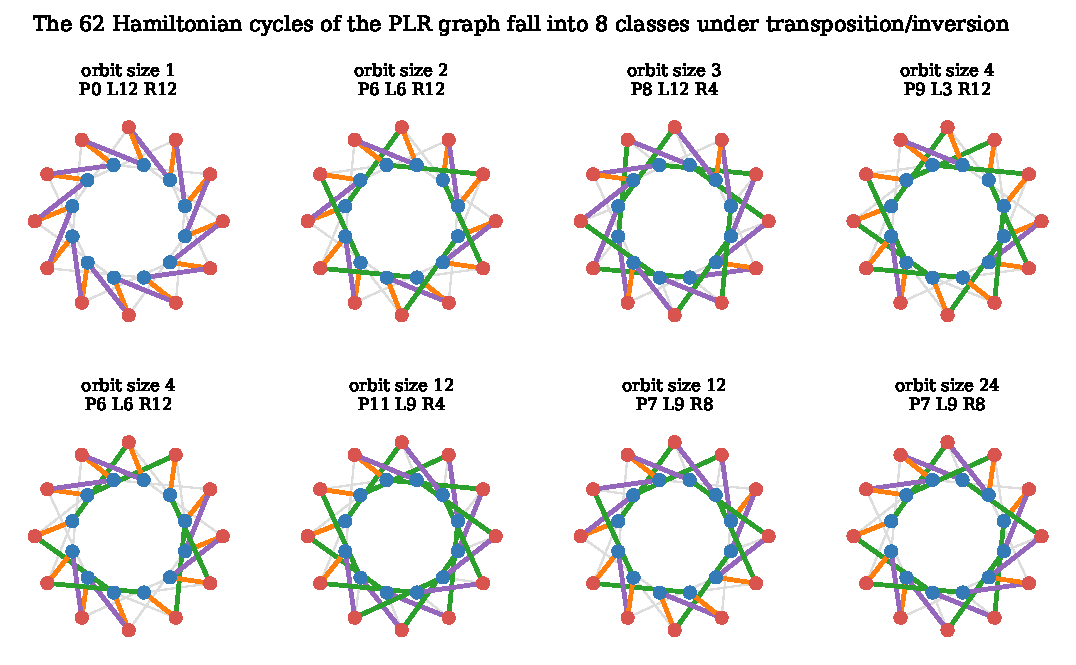
\includegraphics[width=\linewidth]{figures/hamiltonian_classes.pdf}
\caption{One representative of each class. Majors (red) lie on the outer ring ordered by fifths, each relative
minor (blue) just inside. Edge colours: $P$ green, $L$ purple, $R$ orange.}\label{fig:hamclasses}
\end{figure}

\Cref{tab:ham} and \cref{fig:hamclasses} summarise the result. Several observations are worth drawing out.
\begin{enumerate}
\item The $(LR)^{12}$ cycle is the unique cycle fixed by every symmetry. It is the ``circle of fifths with
relatives'': C, Em, G, Bm, D, F$\sharp$m, $\dots$
\item Every cycle uses $R$ at least four times and at most twelve. Because $R$ is the only operation that moves a
voice by a whole tone, the total voice leading ranges from 28 to 36 semitones: the classes of orbit size 3 and 12
with only four $R$ moves are the \emph{smoothest} complete tours of the triads.
\item Two pairs of classes share the same letter counts (6/6/12 and 7/9/8) but differ in word order, so the
letter counts alone do not classify cycles.
\end{enumerate}

\section{Do they sound better?}
The presentation asks whether Hamiltonian cycles sound better than other progressions. The mathematics cannot
answer this, and to our knowledge no controlled perceptual study has addressed it. What can be said is
structural: a Hamiltonian cycle uses maximal harmonic variety (every triad once) with minimal voice leading at every
step, a combination composers have exploited deliberately: Cannas and Andreatta point to pieces by Giovanni Albini and
Moreno Andreatta built on such cycles \citep{cannas2018}. A proper test would compare listener ratings of Hamiltonian cycles
against controls such as random walks on $\Gamma$ (same step size, but with repeats) and random orderings of the
24 triads (same variety, larger steps), matched for tempo, register and voicing. \Cref{ch:outlook} returns to this
as an open project, and \sheet{09\_research\_sandbox.ipynb} generates candidate stimuli.

\begin{notebookbox}
\sheet{04\_hamiltonian.ipynb}: enumerate the cycles, reproduce \cref{tab:ham}, and \emph{listen} to the smoothest
cycle and to the $(LR)^{12}$ cycle, synthesised in the notebook.
\end{notebookbox}

\begin{qa}
\Qu{Reconcile the numbers 62 and 124.}
\A{124 counts directed cycles (a direction of travel is chosen); each undirected cycle gives two directed ones, so
there are 62 undirected cycles.}
\Qu{Why does fixing the start vertex not lose any cycles?}
\A{Every Hamiltonian cycle passes through every vertex, in particular through the chosen start.}
\Qu{What is the orbit size of a cycle whose stabiliser has order 8?}
\A{$24/8=3$ (orbit--stabiliser theorem). This is the third row of \cref{tab:ham}.}
\Qu{Explain why the $(LR)^{12}$ cycle is unique among cycles using only $L$ and $R$.}
\A{$L$ and $R$ are involutions, so a walk using only them must alternate (repeating a letter would return to the
previous triad). The two alternating walks from a given triad are the same cycle in opposite directions, and it
closes only after 24 steps because $RL$ has order 12 on major triads.}
\Qu{Which Hamiltonian cycles minimise total voice leading, and what is the minimum?}
\A{Those with exactly four $R$ moves, the classes of orbit size 3 and 12 (first of the two 12s) in \cref{tab:ham},
with 28 semitones.}
\Qu{Design a control condition for the question ``do Hamiltonian cycles sound better?''.}
\A{For example, random walks of 24 steps on $\Gamma$ (same local smoothness, repeated chords allowed) and random
permutations of all 24 triads (same variety, larger steps), rendered identically and rated blind.}
\end{qa}
